
\subsection{Unsupervised methods} \label{unsupervised}

Among the most commonly used unsupervised methods there are \acrfull{pca} and clustering methods such as \acrfull{hca} and the k-means method.

The \gls{pca} is a statistical procedure whose principal aim is to reduce data dimension, by converting a set of observations of possibly correlated variables into a set of values of linearly uncorrelated variables (principal components). It aims to explain as much data variability as possible with as few principal components as possible. In general, principal components can be computed up to the total number of variables. It can be seen as a method to compute a new coordinate system formed by the latent variables, which is orthogonal, and where only the most informative dimensions are used. Latent variables from PCA optimally represent the distances between the objects in the high-dimensional variable space.

The results of a \gls{pca} analysis include the scores of the supplied data on the principal components (i.e. the transformed variable values that corresponds to a particular data point), the matrix of variable loadings, corresponding to the weights of each original variable on the new coordinates and the standard deviations (or variance) explained by each of the principal components (or cumulative). In this method, it is generally recommended to use mean-centered data, and because it is also sensitive with respect to outliers, robust \gls{pca} can be used \citep{varmuza2009introduction}.

Cluster analysis tries to identify concentrated groups (clusters) of objects, without prior information about any group membership and/or number of clusters. In other words, cluster analysis tries to find groups containing similar objects, and usually one cannot expect a unique solution for cluster analysis. There are two main types of clustering methods, namely hierarchical and non-hierarchical clustering.

In the \acrfull{hca}, objects and partitions are arranged in a hierarchy and represented in a tree-like dendrogram, being a complementary, nonlinear, and widely used method for cluster analysis (\autoref{clustering}). Strategies for \gls{hca} generally fall into two types: agglomerative and divisive clustering. 

\begin{figure}
	\centering
	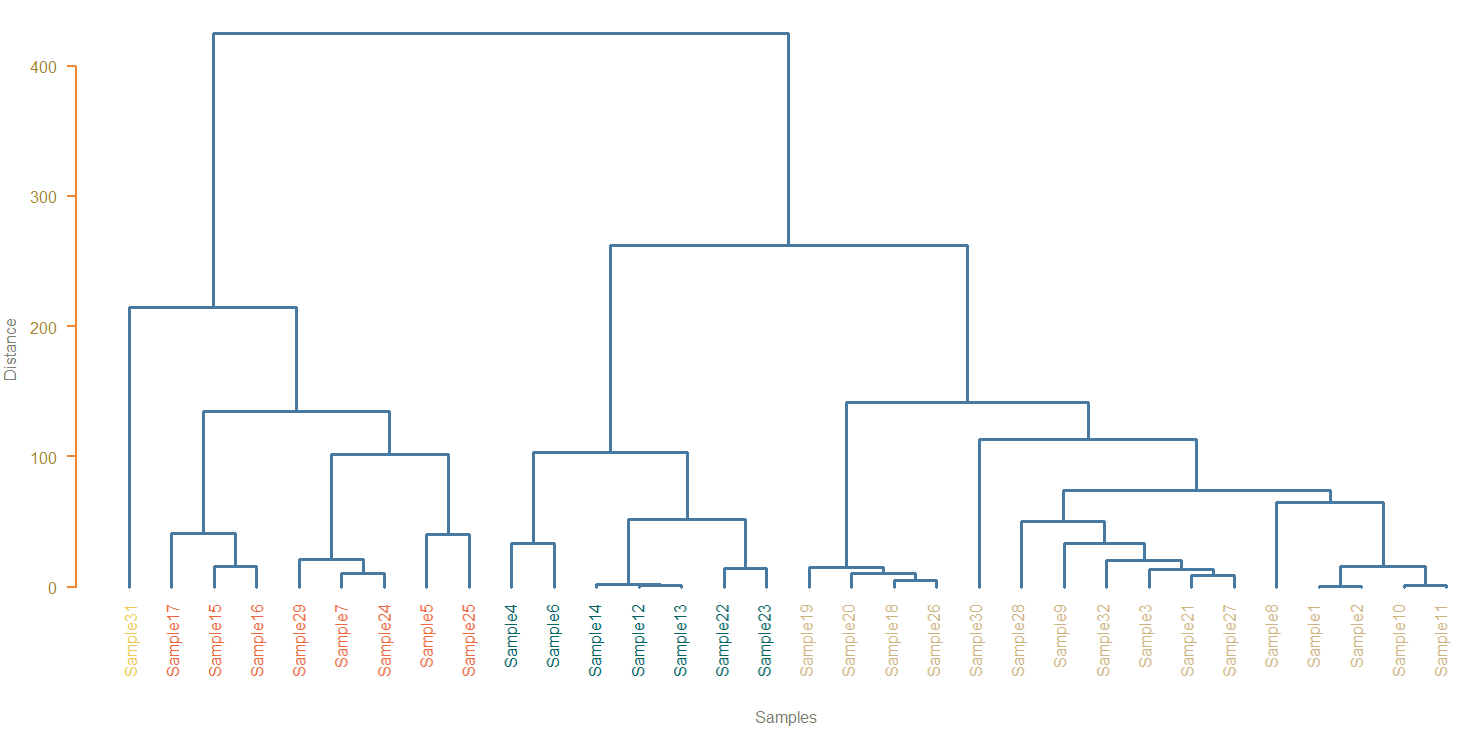
\includegraphics[width=1\linewidth]{Imagens/clustering}
	\caption{Example of a dendrogram resulting from a cluster analysis performed over 32 samples. The distance between samples is represented in the $ y $ axis, whereas sample names are represented in the $ x $ axis.}
	\label{clustering}
\end{figure}


In the first approach, each of the $ n $ objects forms a separate cluster, resulting in $ n $ clusters in the first level. In the next level the two closest clusters are merged, and so on, until finally all objects are in one single cluster. The divisive method groups all $ n $ objects in one single cluster, in the first level of the hierarchy. In the next level, this cluster is split into two smaller clusters, and so on, until finally each object forms a separate cluster. Usually one cannot expect a unique solution for cluster analysis. The result greatly depends on the used distance measure (e.g. Euclidean or Manhattan distances), the cluster algorithm (e.g. Nearest Neighbor or complete linkage), and the chosen parameters \citep{varmuza2009introduction}.

Unlike \gls{hca}, non-hierarchical clustering methods aim to partition a dataset into a pre-defined number of clusters, organizing data objects into a set of typically non overlapping flat groups, by typically using iterative algorithms that optimize a chosen criterion. One of the most used non-hierarchical clustering formulations is the k-means clustering. An algorithm for this approach starts from a set of initial random clusters, then proceeding to take each point belonging  to a  given data set and associate it to the nearest center, minimizing the distance of the observation to the cluster mean. This last step is repeated until no improvement in the objective function can be made. This algorithm (named Lloyd algorithm) is usually fast, however, given that it is an heuristic algorithm, there is no guarantee that it will converge to the global optimum, and the result may depend on the initial set of clusters.




